\chapter{The Relativistic Heavy Ion Collider}

\section{Overview}
While there have been many experiments which have performed deep inelastic
scattering over the years, the experiments built around the Relativistic Heavy
Ion Collider at Brookhaven National Laboratory are positioned to take advantage
of this unique accelerator. 

\begin{figure}[ht]
  \centering
  \begin{subfigure}[b]{\textwidth}
    \centering
    \includegraphics[width=0.8\linewidth]{./figures/kiyoshi_tanida_rhic_schematic.png}
    \caption{Diagram of RHIC Accelerator Complex, (Figure from Kiyoshi Tanida)}
    \label{fig:rhic_schematic} 
  \end{subfigure}
  \begin{subfigure}[b]{\textwidth}
    \centering
    \includegraphics[width=0.8\linewidth]{./figures/7979381212_fddf3f1ab4_z.jpg}
    \caption{Aerial photograph of RHIC Complex \cite{BNLFlickr2011}}
    \label{fig:rhic_aerial}
  \end{subfigure}
  \caption{
		A diagram of the acceleration process of RHIC is shown in the top panel, and
		aerial view is shown in thin the bottom panel. RHIC is nearly four miles in
		circumference and collides a variety of ions at center-of-mass energies
		between $5$ Gev $\sqrt{s}$  and $510$ GeV $\sqrt{s}$.
  }
  \label{fig:rhic_complex}
\end{figure}

The Relativistic Heavy Ion Collider (RHIC) is the world's only intersecting ring
particle accelerator which is capable of colliding polarized proton beams. The
beams are differentiated with the mnemonic ``Blue'' and ``Yellow'' labels. The
blue beam circulates clockwise when viewed from above the RHIC complex, the
yellow beam circulates counter-clockwise. As is typical for intersecting ring
experiments, the beams are bunched, with bunches of ions intersecting at
designated intersection points, around which experiments are built.  The filled
bunches from the blue and yellow beams cross at a frequency of 106 nanoseconds.
PHENIX's timing is set to correspond to the crossing rate of the blue and yellow
beams. Because bunches always collide simultaneously, the blue beam timing clock
is used as a matter of convention, though there are other timing clocks
available for use. The bunches in the beams are numbered as a means of
associating the bunch polarization configuration with the bunch crossing at each
interaction region. This is necessary for any measurement which requires a
knowledge of the initial polarization state of colliding hadrons (such as any
spin physics measurement). This will be discussed more in the section of
discussing the beam polarization at RHIC~\ref{sec:beam_polarization}.

RHIC generally separates data taking into beam `fills' which are uniquely
numbered, and for which general data characterizing the machine state is logged
in various databases and online logbooks. Logging is an important part of data
quality assurance, but also plays a fundamental role in the physics. For
example, the initial spin state of the colliding bunches is logged in databases,
without which, spin analyses are impossible. The trigger configuration is
recorded along with the rates associated with each trigger. Data logged into
logbooks and databases characterizing a fill's performance also plays an
important forensic role with regards to solving issues which occurred during
data taking, but were not immediately caught. Furthermore, because PHENIX is an
international collaboration, this logged data is fundamentally important to
communicating the state of the machine and data collection to the collaboration,
as well as establishing a record of operations.  

RHIC fills are composed of a unique population of bunched ions, circulating
around the rings. During polarized fills, every bunch is polarized according to
a planned polarization pattern. At the end of each fill, (typically 8 hours of
collisions), the beam is dumped, and a new fill is generated.  Experiments built
around RHIC generally subdivide fills into `runs', where a run is a period of
time where the experiment is taking data during which there were no obvious
machine malfunctions. When major issues occur during a run, data taking is
interrupted until the problem is remedied, and the data is discarded. At PHENIX,
runs are always segregated within a fill--no run will ever contain data from
multiple fills, due to the additional complexity of potentially changing machine
conditions, significant down-time between fills, and the potential of beam-dumps
into sensitive high voltage enabled electronics.

Scientists at RHIC have come up with many ingenious ways to create and maintain
beam polarization (Section~\ref{sec:beam_polarization}), once this is
accomplished, various kinematically select probes are engineered, based on
collisions observed which provide important cross-checks to DIS data as well as
original discoveries and measurements of proton structure. RHIC is a unique
collider in that it is quite flexible. Beams may be transversely or
longitudinally polarized, a variety of ions may be used to fill the beams. To
date, RHIC has collided many beam ions and species, summarized in
Figure~\ref{fig:rhic_early_run_summary} and
Figure~\ref{fig:rhic_late_run_summary}.

RHIC is an facility which has been built on top of previous accelerator
experiments--a Linear Accelerator, a booster ring, and an Alternating Gradient
Synchrotron, all of which now have been re-purposed to create the necessary beam
injection conditions appropriate for RHIC. Many experiments are still set up
around various egress points along the acceleration chain, which are publicised
on the Brookhaven National Laboratory website \url{www.bnl.gov}

\begin{figure}[ht]
  \centering
  \includegraphics[width=0.8\linewidth]{./figures/rhic_early_run_summary.png}
  \caption{ 
    Runs 1--3 at RHIC focused on commissioning work for experiments measuring
    collisions at RHIC. Work was mostly characterized by heavy-ion measurements
    related to understanding Quark-Gluon Plasma. The spin program began with Run
    5. Table produced from data posted at the RHIC run page \cite{Fischer2016}.
  }
  \label{fig:rhic_early_run_summary}
\end{figure}

\begin{figure}[ht]
  \centering
  \includegraphics[width=0.8\linewidth]{./figures/rhic_late_run_summary.png}
  \caption{ 
    Though RHIC is currently still running (as of May 9, 2016), I include runs
    here up to and including the run producing my data set (Run 13). An
    unprecedented 13.3 cryo-weeks of running was awarded to the W-Physics
    group.  Table produced from data posted at the RHIC run
    page \cite{Fischer2016}.
  }
  \label{fig:rhic_late_run_summary}
\end{figure}

At the time of writing of this Thesis (Spring of 2016), there are two
experiments which are actively taking data from collisions produced by RHIC: The
Pioneering High Energy Nuclear Interaction Experiment (PHENIX,
Section~\ref{sec:PHENIX}, Figure~\ref{fig:phenix_and_star}), and the Solenoidal
Tracker at RHIC (STAR, Figure~\ref{fig:phenix_and_star}). STAR and PHENIX are
complimentary to each other--PHENIX has a very high precision centrally covering
Electromagnetic Calorimeter, and other high precision detectors, but lacks full
kinematic coverage, whereas STAR has lower precision (with some measurement
dependent exceptions), but has the advantage of nearly full kinematic coverage
around the beam intersection at its center.

RHIC's luminosity and beam polarization has been continuously improving
(Figure~\ref{fig:rhic_luminosity}) since RHIC was first turned on. As we will
discuss later (Section~\ref{sec:forward_upgrade}), the increased luminosity
observed in 2013, was maximally leveraged with upgrades to the PHENIX detector.

\begin{figure}[ht]
  \centering
  \includegraphics[width=0.8\linewidth]{./figures/RhicLuminosityPP.png}
  \caption{
    Upgrades to RHIC's electron lens have enabled massive improvements to
    luminosity--seen in the year 2013. The high luminosity was taken advantage
    of with an extra long proton+proton run. Figure obtained from
     \cite{Fischer2016}
  }
  \label{fig:rhic_luminosity}
\end{figure}


\clearpage
\subsection{Experimental Apparatus}

\begin{figure}[ht]
  \centering
  \includegraphics[width=\linewidth]{./figures/rhic_graphics_fig2-hr.jpg}
  \caption{
    STAR (a) and PHENIX (b) with cutaways showing the event display for a
    heavy-ion collision as reconstructed by the detectors' electromagnetic
    calorimeters~\cite{Walsh2012}.
  }
  \label{fig:phenix_and_star}
\end{figure}

RHIC accelerates ions in a multi-stage process, summarized in
Figure~\ref{fig:rhic_complex}. The source of the beams is the \textbf{Electron
Beam Ion Source}, built on top of a $200$ MeV linear accelerator (Linac). Once
ions are injected into the Linac, they travel to the \textbf{Booster
Synchrotron}.  At this stage, ions are accelerated with pulsed RF fields. After
the beam of ions has been accelerated to nearly the speed of light, they are fed
into the \textbf{Alternating Gradient Synchrotron} or AGS. At this time, ions
are traveling at about 0.37~$c$. By the time the ions leave the AGS, they are
moving at 0.997~$c$. When the ions have reached the appropriate injection energy
(which is ion-species dependent), they are transferred to the
\textbf{AGS-to-RHIC Line}, where a switching magnet pumps bunches of ions into
either the counterclockwise circulating ring of RHIC, or the clockwise
circulating ring of RHIC. The ions are accelerated here to maximum speed--each
beam-ion travels a distance of 2.4 miles every 12.8 microseconds (0.99999~$c$ at
510 GeV $\sqrt{s}$ beam energy), for the duration of a
physics-fill~\cite{RHIC2016}.

When the RHIC rings are filled with ions, the ions are bunched into rotating
electromagnetic potentials called `buckets'. There are 360 beam-buckets in
total, but typically only a fraction are filled with ions. For this analysis, we
took data with beams with 110 filled buckets. The sequence of beam buckets from
one filled bunch to the next is referred to as a `bunch'--and are rather long -
Figure~\ref{fig:bunch_profile_overlay}. The bunch length is 12 meters
longitudinally. The bunch width is quite narrow--with Gaussian geometry, it is
between 150 mm and 300 mm depending on the beam energy.  Understanding the beam
bunch geometry is a crucial component to understanding total the total
luminosity delivered by RHIC to PHENIX. . A detailed presentation of beam
dynamics with regards to luminosity will be presented in chapter
\ref{ch:vernier_analysis}. 

\begin{figure}
  \centering
  \includegraphics[width=0.7\linewidth]{./figures/wcm_16587.jpeg}
  \caption{
		The longitudinal distribution of all bunches in a typical fill are overlaid.
		The bunches from the blue beam (top) and yellow beam (bottom) are shown for
		over a 40 nanosecond time period. 
  }
  \label{fig:bunch_profile_overlay}
\end{figure}

\clearpage
\section{Production of Polarized Proton Beams}

The production of polarized beams is crucial to the physics of this measurement
- without polarized beams, no spin structure analysis can be done at RHIC. This
is due to the fact that the helicity state of the protons in the initial state
of any proton proton collision can be connected to the final observed states in
a way which provides information about the spin structure function, as was
discussed in Section~\ref{ch:modeling_proton_spin}. 

The production of polarized beams is a multistage process, and involves several
experimental components. The importance of polarizing the beams is fully
realized once polarized beams are collided at relatively high center of mass
energies--where the beams behave less like polarized proton beams, but more like
polarized beams of quarks and gluons~\cite{Alekseev2003}. The is produced from a
special polarized ion source, (OPPIS, Figure~\ref{fig:rhic_oppis}). Polarization
is at its maximum at production time, and over the course of the acceleration
through the various apparatuses described below, we work to maintain
polarization by limiting and mediating depolarizing resonances,
Figure\ref{fig:rhic_complex}. The exact details of beam injection and
polarization management is presented in the RHIC Configuration
Manual~\cite{RHIC2006}, with the relevant portions summarized here.

\subsection{Polarized Injection}

RHIC uses an optically pumped polarized ion source (OPPIS),
Figure~\ref{fig:rhic_oppis} to produce a polarized ion source greatly in excess
of RHIC's design intensity. This is used to our advantage, as the emittance of
the beam can be lowered to create a highly collimated beam for physics use.

\begin{figure}[ht]
	\centering
	\includegraphics[width=0.8\linewidth]{./figures/rhic_oppis.png}
	\caption{
		RHIC's optically pumped polarized ion source. Produces 0.5-1.0 mA current of
		polarized $H^-$ ions. The optical pumping is pulsed at 400
		$\mu$s, \cite{Zelenski2007}
	}
	\label{fig:rhic_oppis}
\end{figure}

\clearpage
\subsection{AGS to RHIC Transfer Line}

\begin{figure}
  \centering
  \begin{subfigure}[b]{\textwidth}
    \centering
    \includegraphics[width=0.7\linewidth]{./figures/rhic_polarized_injector.png}
		\caption{
			Technical schematic of Polarized Injection Line \cite{Zelenski2007}
		}
    \label{fig:polarized_top_view_1} 
  \end{subfigure}
  \begin{subfigure}[b]{\textwidth}
    \centering
    \includegraphics[width=0.7\linewidth]{./figures/polarized_beam_rhic_complex.png}
		\caption{
			Overhead view of Polarized Injection Line \cite{RHIC2006}
		}
    \label{fig:polarized_top_view_2}
  \end{subfigure}
  \caption{
    A view of the RHIC polarized injection system. Panel (a) shows a zoomed in
    technical view of the OPPIS to the booster. Panel (b) shows a zoomed out
    cartoon of the next step in the polarization injection system, including
    the AGS, and the feeder line to RHIC.
  }
  \label{fig:rhic_polarized_beam_line}
\end{figure}

Once ions have been optically pumped, we have a direct-current beam at
approximately 80\% polarization. This is accomplished using optically pumped
Rubidium vapor. The polarized ions are then moved into the booster from the
Linac, where some polarization is lost to spin precession, intrinsic to
accelerating charged ions in a circular path.  However, polarization is
maintained, for the most part, by matching the precession resonance to the
orbiting frequency of the booster ring.  The Siberian snakes
(Section~\ref{sec:siberian_snakes}) at this stage serve to incrementally flip
the ion spin such that the natural depolarization works to re-polarize the
orbiting ions, every full-turn. The full details of this procedure are well
described in Reference~\cite{RHIC2006}.

After the ions are sufficiently polarized and filled in the AGS, they are moved
into the AGS to RHIC Transfer line, Figure~\ref{fig:ags_to_rhic}. The beam is
focused and fed through a switching magnet--which must be timed with great
precision in order to fill the blue and yellow beams with the appropriate
polarization patters. In fact, the precision is so great, that the Earth's
curvature must be taken into account over this relatively short injection line.
The entry point and exit point are bent ever-so-slightly due to the curvature of
the Earth, with the entry being 12.51 mrad and the egress being 12.46 mrad
\cite{RHIC2006}.  At the point of injection in the transfer line, the beam size
and emittance are measured, as well as the beam polarization. 

\begin{figure}
  \centering
  \includegraphics[width=0.6\linewidth]{./figures/ags_to_rhic_transfer}
  \caption{
    A schematic of the geometry of the AGS-to-RHIC transfer line~\cite{RHIC2006}.
  }
  \label{fig:ags_to_rhic}
\end{figure}

\clearpage
\section{Maintaining Beam Polarization}
\label{sec:beam_polarization}

The creation of polarized beams is only half the battle. Depolarizing resonances
in any particle beam are intrinsic in the design of any circulating beam
particle accelerator--without intervention, after a few rotations, RHIC's
polarized beams would be unpolarized. RHIC uses several strategies in concert to
correct for the largest of these depolarizing resonances--including beam orbit
corrections, the Siberian Snakes, Betatron Tune Spreading, and sextupole
magnetic depolarizing resonances. 

\subsection{Siberian Snakes and Spin Rotators}
\label{sec:siberian_snakes}

The Siberian Snakes are positioned at two locations on the RHIC ring (as well as
others along the injection sequence). The most stable configuration of spin
injected in RHIC is such that the spin axis is perpendicular to the plane of the
accelerator ring. The Siberian snake is a helical magnet which forces the spin
to rotate 180 degrees every half rotation. This special configuration of snakes
(see Figure~\ref{fig:rhic_complex}) ingeniously takes advantage of the
rotational precision of the spin (a depolarizing resonance) to re-polarize the
beam, every half-orbit.

The spin rotators are located outside of experimental interaction regions around
PHENIX and STAR. These special dipole magnets rotate the spin of the beams onto
a longitudinal (parallel with beam) axis--these magnets are important for any
measurement (such as this one) requiring longitudinal spin polarization.
Transverse spin polarization has also been used in RHIC operations to probe the
transverse spin structure of protons. It is a complementary and vital area of
inquiry, but is not presented in this work. 

\subsection{Measuring Beam Polarization}

The RHIC Collider-Accelerator Department provides several means of measuring the
beam polarization over the course of the data taking period. PHENIX takes
special data runs which are used to determine the real beam polarization
delivered to the detector, in a yearly analysis. This analysis is referred to
``Local Polarimetry'', or ``LPol''.

CAD will additionally measure polarization in via inelastic proton-carbon
scattering in the Coulomb-Nuclear Interference (CNI) region. Relative
polarization can be determined with to within 10\% in only a few seconds of
measurement. 

Vertical polarization is determined through the calculation of the left and
right particle production, with a known analyzing power (\cite{RHIC2006}, Ch 8):

\begin{equation}
  P_B = {{1}\over{A_p}}{{N_L-N_R}\over{N_L+N_R}}
  \label{eq:rhic_polarization}
\end{equation}

Where $P_B$ is the beam polarization, $N_L$ and $N_R$ are the left-scattering
produced particles, and right-scattering produced particles and $A_p$ is the
analyzing power, which can be calculated from first principals, and
experimentally verified. Scattering takes place as a carbon filament is swept
across the beam.

As many decisions are financially constrained, this one was too. Using a
p-Carbon CNI polarimeter provides an economically viable way to measure beam
polarization within the precision needed for the spin experiments.

\subsubsection{The Spin Monitor}
\label{sec:the_spin_monitor}

During a RHIC run, it is crucial to keep track of the polarization patterns
being collided at the PHENIX IR~\ref{fig:phenix_spin_collision}. 

One of my major contributions to the PHENIX experiment was in the upkeep and
development of the spin monitoring systems for the online data taking portions
of the experiment, show in Figure~\ref{fig:spin_monitor}.


\begin{figure}
  \centering
  \includegraphics[width=\linewidth]{./figures/phenix_spin_collision}
  \caption{
    This cartoon illustrates one potential polarization pattern configuration
    of the beams as they collide at PHENIX's interaction region.  As beams are
    longitudinally rotated into position for collision, it is crucial to keep
    careful track of the magnet currents rotating the beams, as well as the
    overall polarization pattern.
  }
  \label{fig:phenix_spin_collision}
\end{figure}

The spin monitor's purpose is to provide real-time feedback on the dipole
magnets used to orient proton spin orientation prior to collision, as well as
comparing the RHIC spin fill pattern against the measured spin pattern delivered
to the PHENIX interaction region. 

\begin{figure}
  \centering
  \includegraphics[width=\linewidth]{./figures/SPINMON_shift_358904.png}
  \caption{
    The shift-crew display output for the Spin Monitor. The upper panel shows
    the polarization of the blue and yellow beams, and other panels summarize
    information including magnet currents (needed to understand the spin
    orientation), issues with data packet loss, the recognized spin-pattern, as
    well as a large boxed area on the lower left where errors could be shown to
    the shift crew along with the proper response.
  }
  \label{fig:spin_monitor}
\end{figure}

\clearpage
\section{The Pioneering High Energy Nuclear Interaction Experiment}
\label{sec:PHENIX}

The Pioneering High Energy Nuclear Interaction Experiment (PHENIX) is a
synthesis of many smaller detectors all of whom were commissioned for various
physics goals, some of whom have been repurposed from their original
application once its primary physics was completed. PHENIX has several major
physics thrusts, which are discussed below. 

Much of PHENIX collaboration's early published work focused on creating and
studying quark gluon plasma in heavy ion collisions, but in following years
spin papers came too. Major question in physics that PHENIX set out to answer
with its heavy-ion program include studying confinement--i.e.  why are quark
color charges confined to exist in the nucleus, baryons and mesons? PHENIX
sought to study this via examination of the J/$Psi$ and measuring screening
length in heavy ion collisions. Additional research topics included the study
of chiral symmetry restoration, thermal radiation of hot gasses, QCD Phase
transition, Strangeness and Charm Production, Jet Quenching, and Space-time
evolution~\cite{Nagamiya1994} .

The remaining physics goal of the PHENIX collaboration is to study the origins
of proton spin. The PHENIX spin program `officially' started with the RHIC
upgrade to enable production of polarized proton beams. 

The spin program came shortly after the 2001 commissioning run. The first
polarized proton run was produced by RHIC for PHENIX in 2002, with 8.3 total
weeks of data. Data was taken over several discrete periods, as RHIC was still
being optimized for spin physics.

The purpose of the PHENIX spin program has been to understand the spin
structure of the proton, and has historically used various particle production
asymmetries (left-right and forward-backward) as an experimental probe for
polarized parton distribution functions (as discussed in
Chapter~\ref{ch:modeling_proton_spin}). 

PHENIX studies the proton spin structure as modeled by the Ellis-Jeffe sum rule
(Chapter~\ref{ch:modeling_proton_spin}). The PHENIX spectrometer is
particularly well suited to studying gluon polarization, $\Delta g$ and the
anti-quark polarization, $\Delta \bar{q}$. Additionally, the `nature of parity
non-conservation itself can be directly studied'
~\cite{PHENIXCollaboration1998} using polarized beams, and spin asymmetries in
collisions.  This measurement requires a means of reconstructing jets,
inclusive or leading particle production can be used as a proxy with some small
asymmetry remaining.

The configuration of the PHENIX spectrometer changes from year to year, as part
of planned upgrades. The configuration of the detector for the 2013 physics run
is shown in Figure~\ref{fig:phenix_2013_config}.

\begin{figure}
  \centering
  \begin{subfigure}[t]{\textwidth}
    \centering
    \includegraphics[width=0.8\linewidth]{./figures/phenix_2013_config_central_arms}
    \caption{Central Arms}
    \label{fig:phenix_central} 
  \end{subfigure} 
  \begin{subfigure}[t]{\textwidth}
    \centering
    \includegraphics[width=0.8\linewidth]{./figures/phenix_2013_config_muon_arms}
    \caption{Forward Muon Arms}
    \label{fig:phenix_forward}
  \end{subfigure}
  \caption{
    Shown: The two main arms of the PHENIX Spectrometer. The central arms are
    shown via the beam-on view of PHENIX (a) and Forward Muon Arms are highlighted
    via the 90-degree rotated view (b). In both cases, the 2013 configuration is
    shown. The beams are brought into intersection at the geometric center of
    each figure (immediately between the BBCs)
  }
  \label{fig:phenix_2013_config}
\end{figure}

PHENIX makes use of many classic detectors, including  Cherenkov light
detectors, resistive plate chambers, electromagnetic calorimeters, silicon chip
detectors, time of flight detectors, scintillation light detectors, cathode
strip chambers, and proportional tube counters.

While all of these subsystems are interesting, and have produced excellent
physics results, I will focus only on those pertinent to this analysis.

PHENIX is generally thought of as two `halves' being comprised of two broadly
defined `arms'--the forward muon arms, and the central arms. As the names
suggest, the central arms cover the central rapdity range (close to $y=0$),
whereas the muon arms cover larger rapidities and specialize in detecting muons.
While both kinematic regions are used for heavy ion and spin physics analyses,
this analysis exclusively uses the forward muon and the Beam Beam Counters. The
majority of the central arms systems will not be discussed in detail in this
thesis.

\subsection{Units}

The data taken by PHENIX as well as the geometry of the detector can be
characterized by various measurements and units. The data taken by the detector
is shown relative to the PHENIX Coordinate System
(Figure~\ref{fig:phenix_coordinate_system}). Some accelerator-specific units
are summarized in Table~\ref{tab:units}. The full description of the data taken
by PHENIX is saved for Chapter~\ref{ch:data_analysis}.

\begin{figure}[ht]
  \centering
  \includegraphics[width=\linewidth]{./figures/phenix_coordinate_system.png}
  \caption{
    The PHENIX coordinate system is shown (RGB arrows) at the center of the
    nominal interaction point within PHENIX, the origin, in this quarter-cutaway
    drawing. The small black figures are actually miniaturized human beings, the
    PHENIX detector is very small--this is a full scale drawing of PHENIX.
    Shown: the x, y, and z coordinates, as well as the azimuthal coordinate,
    $\theta$ and polar coordinate $\phi$ ~\cite{WebPHENIXDrawings}
  }
  \label{fig:phenix_coordinate_system}

\end{figure}

\begin{table}[ht] 
  \centering
  \begin{tabular}{ c c p{8cm} }
    \toprule
    \textbf{Quantity} & \textbf{Definition} &  \textbf{Description} \\
    \midrule
    $x,y,z$ & & Cartesian coordinates whose origin is at the center of the PHENIX spectrometer. \\
    $\theta$ & & Polar coordinate relative to origin of PHENIX coordinate system describing angle between the positive z-axis and a reference point \\ 
    $\phi$ & & Polar coordinate relative to the origin of the PHENIX coordinate system describing the angle between a reference point and the x-axis \\
    $v$ & & Speed of a particle \\
    $c$ & & Speed of light \\
    $E$ & & Relativistic energy of a particle \\
    $p$ & $\left(p_x,p_y,p_z,E\right)$ & Total four-momentum of a particle \\
    $y$ & $tanh^{-1}(v/c)$, ${1\over2}{ln{{E+p_zc}\over{E-p_zc}}}$ & Spatial coordinate, rapidity, describing the hyperbolic angle differentiating between two frames of reference in relative motion. When described in terms of $E,p_z$, $y$ describes the relativistic boost along the z-axis of the beam\\ 
    $\eta$ & $-ln\left[tan\left({\theta\over2}\right)\right]$ & Spatial coordinate describing the angle of a particle relative to the beam axis \\
    \bottomrule
  \end{tabular}
  \caption{
    Some units describing the geometry of and data taken by PHENIX.
  }
  \label{tab:units}
\end{table}

A closely related analysis measures $W\rightarrow e$ processes uses the central
arms. As different arms are sensitive to different rapidity ranges,
complimentary results are obtained from central and forward analyses. The
central analysis is presented in References \cite{Gal2014b} and
\cite{Adare2015a}. 

PHENIX also utilizes a complex data acquisition system (DAQ) which streams data
from each detector, assembles this data into a labeled event, compresses and
finally stores into a proprietary storage format. The work-flow of the DAQ is
summarized in Figure~\ref{fig:phenix_daq_overview}. 

For each event, any particles which interact with the detector material are
transduced by. The transduced signals are serialized into a detector-specific
data stream, such that the state of the detector's excitation can be recorded
and reproduced later. This information is stored on the front-end-electronics
modules (FEMs), and synchronized with timing information from the clock (ticks
once every time there is a bunch crossing) and a Global Trigger decision, i.e.
whether or not the right parts of the detector lit up to make this particular
event worth keeping. If the detector triggering heuristics determine that an
event is worthy of keeping, the uncompressed serialized information is sent to
the DCMs (Data Collection Modules), where it is assembled into a packet, and
then sent to the event builder (EvB). At the EvB, all packets originating from a
common collision are assembled into an event.  The event is compressed into a
proprietary PRDF (PHENIX Raw Data File Format) format, and sent to the Buffer
Boxes, a cache of high density local storage. Finally, this cached data is sent
off to high density, robotic magnetic tape storage on magnetic for ultra-stable
archival. Later, this data is copied to a computing cluster, and reconstructed
into `analysis-ready' data structures, such as track reconstruction variables,
event vertices and so-on. This is discussed in Chapter~\ref{ch:data_analysis}
and Chapter~\ref{ch:feature_engineering}.

A complete summary of PHENIX detector subsystems (excluding the new Forward
Vertex Detector, Silicon Vertex Detector, and Resistive Plate Chambers, which
discussed separately) can by found in Table~\ref{tab:phenix_detector_summary}.

\begin{figure}
  \includegraphics[width=\linewidth]{./figures/daq_overview}
  \caption{ 
    Shown: A flow chart summarizing the PHENIX DAQ \cite{Desmond2016}. 
  }
  \label{fig:phenix_daq_overview}
\end{figure}

\begin{table}
  \centering
  \begin{tabular}{l c c p{5cm}}
    \toprule
    \textbf{Element}	& \textbf{$\eta$}	& \textbf{$\phi$} & \textbf{Features} \\
    \midrule
    \textbf{Magnets}  & & & \\
    Central Magnet    & $ \vert\eta\vert < 0.35$ & $360^{\circ}$ & 1.15 $T$ \\ 
    Muon Magnet North & $1.1 < \vert\eta\vert < 2.2$ & $360^{\circ}$ & 0.72 $T$ \\
    Muon Magnet South & $1.1 < \vert\eta\vert < 2.4$ & $360^{\circ}$ & 0.72 $T$ \\
                      & & & \\
    \textbf{Minimum Bias} & & & \\
    Beam Beam Counter & $(3.1 < \vert\eta\vert < 3.9)$ & $360^{\circ}$ & Vertex Reconstruction \\
    Zero Degree Calorimeter & $\pm 2 mrad$ & $360^{\circ}$ & Minimum Bias Trigger \\
                            & & & \\
    \textbf{Central Detectors} & & & \\
    Drift Chambers & $\vert\eta\vert < 0.35$ & $90^{\circ}\times2$ & Central $p$ and $m$ resolution \\
    Pad Chambers & $\vert\eta\vert < 0.35$ & $90^{\circ}\times2$ & Pattern Recognition, Tracking \\
    Ring Imaging Cherenkov & $\vert\eta\vert < 0.35$ & $90^{\circ}\times2$ & Electron ID \\
    Time of Flight & $\vert\eta\vert < 0.35$ & $45^{\circ}$ & Hadron ID, $\sigma<100pm$ \\
    PbSc EMCal & $\vert\eta\vert < 0.35$ & $90^{\circ}$, $45^{\circ}$ & Calorimetry, photon, and electron energy \\
    PbGl EMCal & $\vert\eta\vert < 0.35$ & $45^{\circ}$ & $e^{\pm}$, $\mu^{\pm}$ separation at $p> 1 GeV/c$ EM Shower and $p < 0.35 GeV$, $K^{\pm}$ $\pi^{\pm}$ separation up to $1 GeV/c$ \\
    \textbf{Muon Arms} & & & \\
    Muon Tracker South & $1.15 < \vert\eta\vert < 2.25$ & $360^{\circ}$ & North installed 2003 \\
    Muon Tracker North & $1.15 < \vert\eta\vert < 2.44$   & $360^{\circ}$ &  \\
    Muon ID South & $1.15 < \vert\eta\vert < 2.25$ & $360^{\circ}$ & Steel absorbers, larocci tubes \\
    Muon ID North & $1.15 < \vert\eta\vert < 2.44$   & $360^{\circ}$ & "" \\
    \bottomrule 
  \end{tabular}
  \caption{
    A summary of PHENIX hardware~\cite{Adcox2003}. $e^\pm$/$\pi^\pm$ separation
    and $\pi$/$K$ separation requires the Time of Flight (ToF) working with
    PbGl and PbSc data. PbGl refers to ``Lead Glass Scintillator'' and PbSc
    refers to ``Lead Scintillator''. The Muon Identifier (Muon ID, MuID) can
    help suppress hadrons by absorbing them in the iron layers. 
  }
  \label{tab:phenix_detector_summary}
\end{table}

\clearpage

\subsection{Subsystems}

The major subsystems contributing to this work include the Muon Arms, the Beam
Beam Counters (BBCs), and the Forward Vertex Detector, since the analysis is
characterized by calculating the asymmetry for $W\rightarrow\mu$ interactions,
only muon reconstruction and identification is required. For the complimentary
central arm analysis, the $W\rightarrow e$ decay mode is explored.

\subsubsection{Beam Beam Counters}

The Beam-Beam counters (BBCs, Figure~\ref{fig:bbc_overview}) are
photomultiplier tubes with scintillating lead-glass crystals. These detectors
are situated 144 cm from either side of the nominal center of the PHENIX
interaction region. The primary purpose of the BBCs is to provide the time of a
beam-beam collision for triggering, and to measure the Z-Vertex of the
collision (Figure~\ref{fig:bbc_zvertex_example}).

\begin{figure}[ht]
  \centering
  \includegraphics[width=0.7\linewidth]{./figures/bbc_zvertex}
  \caption{
    Here, we see a typical BBC z-vertex distribution for one run's worth of
    data, over a z-vertex range of -300 cm to 300 cm. The central peak is close
    to the nominal interaction point of z = 0 cm. The peaks to the left and
    right (at $\pm$144 cm) are from collisions outside of the BBC.
  }
  \label{fig:bbc_zvertex_example}
\end{figure}

When a collision occurs, each BBC measures the arrival time of the leading
charged particles, $T_S$ for the south BBC, and $T_N$ for the north BBC
(Figure~\ref{fig:bbc_vertex_reconstruction}). These times are defined as the
average of times within the established timing window - each element of the BBC
is capable of 52$\pm$4 ps, which is a factor of \~2500 less than the bunch
crossing rate (1 bunch every 106 ns)~\cite{Allen2003}.

The Z-Vertex is determined from $T_N$ and $T_S$ as follows:

\begin{equation}
  Z_{vertex} = c * (T_S - T_N) / 2.0
  \label{eq:zvtx_calc}
\end{equation}

Note that a consequence of the way the z-vertex is calculated, when there are
collisions occurring are outside of the BBCs (i.e. $-144 cm > z_{vertex}, z_{vertex}
> 144 cm$), the reconstructed z-vertex will either be at 144 cm or -144 cm.
These events are removed with a vertex cut on the data.

The BBCs are used to record data with minimal bias towards any events
containing any particular physics characteristic. This is important as a means
for reconstructing the absolute abundance of particle production, which is
crucial for determination of any inelastic scattering cross section and
normalization of any cross-section of interesting scattering events.  The
Beam-Beam counters provide a measurement of vertex reconstruction by way of
analyzing the time delay between triggering of the North and South BBCs.  The
delay window is then used to reconstruct the event vertex by assuming the
impinging particles were traveling at near the speed of light,
Figure~\ref{fig:bbc_vertex_reconstruction}. 

\begin{figure}[ht]
  \centering
  \includegraphics[width=\linewidth]{./figures/bbc_overview.pdf}
  \caption{
    Shown: a schematic of the exact proportions of the detector as viewed
    alongside the beam pipe, along with the pseudorapidity and azimuthal
    coverage~\cite{Nakamura2002}
  }
  \label{fig:bbc_overview}
\end{figure}

\begin{figure}[ht]
  \centering
  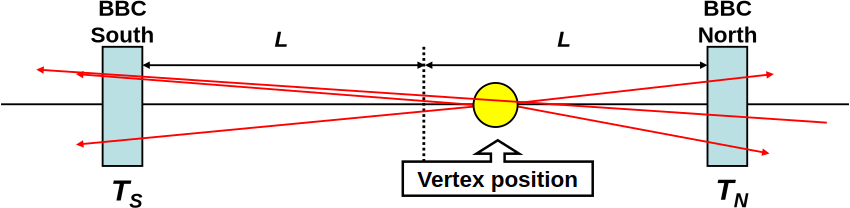
\includegraphics[width=\linewidth]{./figures/bbc_vertex_reconstruction.pdf}
  \caption{
    Showers from the primary event vertex impinge on the north and south BBC.
    The average timing of these particles are used to calculate $T_N$ and $T_S$,
    allowing for the calculation of event z-vertex (Equation~\ref{eq:zvtx_calc})
  }
  \label{fig:bbc_vertex_reconstruction}
\end{figure}

\clearpage
\subsubsection{Forward Vertex Detector}

The Forward Vertex Detector (FVTX), Figure~\ref{fig:forward_vertex_detector} is
a silicon detector, which enables detection of secondary event-vertices.  This
provides additional information to improve the precision to the Muon Tracking
system. As a result of this improvement, secondary vertices can be measured
allowing the distinction of particles decaying at the primary event vertex. 

For this analysis, the FVTX can provide an important additional layer of
precision, because it can help to identify background-events which do not
originate from the primary event vertex of a collision~\cite{Aidala2014}.  

\begin{figure}[ht]
  \centering
  \includegraphics[width=0.6\linewidth]{./figures/forward_vertex_detector}
  \caption{
    A schematic of the Forward Vertex Detector, showing the silicon chip layers
    (light blue wedges), and readout electronics (green). The FVTX was designed
    to mount directly onto the Silicon Vertex Detector
    (center)~\cite{Aidala2014}.  This configuration allows for a very high
    density of interleaved chips, in several layers, covering a maximum area
    around the beam pipe for detection of secondary vertex events. Secondary
    vertices are expected to occur rapidly after the primary vertex, making the
    region close to the primary vertex important real-estate to occupy.
  } 
  \label{fig:forward_vertex_detector}
\end{figure}

\edithere{}

\clearpage
\subsubsection{The Muon Arms}

The Muon Arms are composed of several subsystems, including the Muon Tracker
(MuTR, cathode strip chambers), the Muon Identifier (MuID, shielding and
scintillation layers), and the Resistive Plate Chambers (RPC(s), bakelite gas
gaps and azimuthal oriented capacitively coupled copper readout strips). The job
of the muon tracker is to identify muons with the penetration through the many
layers of the MuID, and provide momentum and charge reconstruction for muon
tracks. Tracks are matched to the event vertex with Kalman filter during
reconstruction, and can even be matched with FVTX secondary vertices as a means
of rejecting non W-Boson decays. Prior to the Forward Upgrade
(Section~\ref{sec:forward_upgrade}), the muon arms consisted solely of the Muon
Tracker and the MuID. 

The Muon Tracker has a radial magnetic field, leading to charged particles
traversing the tracker to have a helical bend. This was suitable for lower
energy muon tracks, such as muons coming from the J$\Psi$ decay, which was one
of the primary decays targeted in the original design of the muon tracker.

However, these J/$\Psi$ muons have much lower energy then muons which decay from
areal W-Boson production. To extend the muon tracker's usefulness into tracking
these high energy muons, an upgrade to the triggering system was required to
obtain adequate back-ground rejection for the Forward W analysis. The details of
the muon arms will be discussed in the next section.

\clearpage
\section{The Forward Upgrade} 
\label{sec:forward_upgrade}

The muon arms were the subject of significant upgrades from 2011-2013.
New front end electronics were added to improve triggering, and entire new
detector subsystems (The RPCs) were added. The full details of these subsystems
will be discussed in the forthcoming sections (Section~\ref{sec:forward_upgrade}).

One of the main stated physics goals of PHENIX is to constrain the sea-quark
polarization of the proton spin. While this contribution is
expected to be small, it is not because it is expected to be uniformly zero.
Instead, the expectation is that the matter contribution to the quark sea is
strongly positively polarized, while the antimatter contribution is strongly
negatively polarized~\cite{Aidala2005}. Measuring this polarization via $A_L$
(Equation~\ref{eq:w_production_asymmetry}) is the means by which we will
accomplish this. Prior to the Forward Upgrade, we only had results from the
Central $W\rightarrow\mu$ analysis, but to better constrain our models, we
require lower uncertainty in the forward kinematic regime--thus, the Forward
Upgrade.

The first data for this measurement was taken in 2009, and published in 2010
under \cite{Adare2010} and \cite{Okada2010}, but only for central rapidities,
where a clear Jacobean peak could be found in the electron invariant mass
spectrum at 40$GeV$ mass-energy (half the rest mass of the W-Boson). This made
evaluating yields and calculating asymmetries relatively straight-forward. 

However, in forward kinematic regimes, it was very difficult to discriminate
real $W\rightarrow\mu$ from other sources $X\rightarrow\mu$. As one can observe
in Figure~\ref{fig:muon_production_vs_pt}, only at high $p_T$ does the W-boson
signal become dominant. The old muon trigger electronics did not allow
triggering sufficiently close to the W-Boson production threshold to allow for
enough data to be taken. This is because of how the Muon Tracker identifies the
charge and momentum of particles--which is via track bending. As tracks become
very straight (i.e. high $p_T$), the muon tracker struggles to reconstruct the
correct charge and momentum. The original Forward Upgrade called for a nose-cone
calorimeter, which would have helped greatly for particle rejection, but was
canned for budget reasons.

The Forward Upgrade to PHENIX increased the muon triggering threshold from about
2 $GeV$ to 10 $GeV$, enough to insure that all muons produced from W-Boson
decays can be recorded, with no loss of statistics. This of course is not to
say, that these events were recorded without any background processes--the
removal of the muon background was a substantial effort in this analysis,
described in Section~\ref{sec:sbr}.

\begin{figure}[ht]
  \centering
  \begin{subfigure}[b]{0.5\textwidth}
    \centering
    \includegraphics[width=\textwidth]{./figures/w_old_trigger.png}
    \caption{The original Muon Trigger Threshold}
    \label{fig:trig_muon_old}
  \end{subfigure}%
  ~
  \begin{subfigure}[b]{0.5\textwidth}
    \centering
    \includegraphics[width=\textwidth]{./figures/w_dominant_region_new_trigger.png}
    \caption{Muon Trigger Threshold, Forward Upgrade}
    \label{fig:trig_muon_new}
  \end{subfigure}
  \caption{ 
    Observing the simulated production of muon as a function of $p_T$, we can
    see that in the kinematic region of $W$ production that the dominant sources
    of muons come from other processes. The new PHENIX muon trigger threshold is
    sensitive at 10 $GeV/c$ and above. The threshold is still high enough that
    with other methods, we can record all events which come from the W boson,
    with triggering, whereas with the old threshold, this was impossible.
  }
  \label{fig:muon_production_vs_pt}
\end{figure}

\subsection{The Muon Tracker}

The primary purpose of the Muon Tracker is to reconstruct the energy and
momentum of muons in the forward kinematic regime. Because the MuID is composed
of larocci tubes sandwiched between solid steel sheets, only particles which
penetrate all the layers of the MuID are identified as muons. The Muon Tracker
has three cathode strip tracking planes in a volume of gas, with an applied
radial magnetic field. Each plane has two faces of tracking strips, for six
total tracking readouts total. The arrangement of cathode strips  makes the Muon
Tracker very sensitive to the azimuthal dimension, but coarsely sensitive to the
radial direction. The Muon Arms have three tracking stations for momentum and
charge identification, sandwiched between two RPCS.

Since the MuID will fire on Muons with a 2.5 $GeV$ momentum threshold, it will
trigger very rapidly at high beam energies and luminosities--too fast to record
all data--event rates were in excess of 10 MHz in 2013, with only 2 kHz of DAQ
bandwidth allocated to the W analysis. Thus, before the Forward Upgrade, the
Muon Arms were insufficient. However, additional absorber was installed at the
nose-cone of the muon tracker to block lower momentum particles. The addition of
the RPCs as well as new Front End Electronics Modules allowed for the real-time
calculation of pseudo-momentum to be fed into the trigger decision in order to
provide high rejection power on tracks. These upgrades allowed us to trigger
exclusively on relatively straight tracks, which is consistent with high
momentum particles~\cite{Fukao2011}.

\clearpage
\subsection{The Resistive Plate Chambers}

One of my major contributions to the PHENIX experiment was in the construction
and testing of the RPCs at station 1, in 2012. An exploded view of the RPC is
shown in Figure~\ref{fig:rpc_exploded}. The RPCs were a crucial part of the
W-Physics muon trigger. One primary feature the presence of RPCs add to the
PHENIX triggering system is timing resolution--2 nanoseconds
(Table~\ref{tab:rpc_design_characteristics}). This is crucial, because before
the inclusion of RPCs, the only timing available was that of the BBCs. However -
because the BBCs are minimally biased--they will fire nearly every time there
is a collision--which at high luminosity is far greater than the assigned
bandwidth to the W Physics trigger. The RPC provides local timing information,
which allows the triggering system to record events which trigger the muon arm
system, and not just the BBCs. This has the effect of significantly reducing
backgrounds--by a factor of $>$ 6000~\cite{Fukao2011},
Figure~\ref{fig:rpc_rejection_power}.

\begin{figure}
  \centering
  \includegraphics[width=0.8\linewidth]{./figures/rejection_power.png}
  \caption{
    In 2013 with the final commissioning of the RPCs and the Forward Upgrade
    complete, we saw a drastic increase in rejection power, as planned.
  }
  \label{fig:rpc_rejection_power}

\end{figure}


\subsubsection{Design}

\begin{figure}
  \centering
  \begin{subfigure}[b]{0.4\textwidth}
    \centering
    \includegraphics[width=0.8\linewidth]{./figures/rpc_1_muon_hit}
    \caption{A muon passing through the layers of the RPC}
    \label{fig:rpc_hit_side_view}
  \end{subfigure}%
  ~
  \begin{subfigure}[b]{0.4\textwidth}
    \centering
    \includegraphics[width=0.8\linewidth]{./figures/rpc_1_muon_hit_side}
    \caption{Copper readout strip activated by passing muon}
    \label{fig:rpc_hit_top_view}
  \end{subfigure}
  \caption{
    As a muon passes through the layers of the RPC (left), the gas in the
    bakelite gap is ionized. This charge migrates and collects near the highly
    resistive graphite coating. An image distribution is induced on the
    overlapping readout strip (right), which is passed along its own channel to
    the front-end electronics.
  }
  \label{fig:muon_hit_rpc}
\end{figure}

As hinted at prior, the design goal of the Resistive Plate Chambers is to
provide accurate timing information at high speed in order to build a Trigger
which can record $W\rightarrow\mu$ events. RPCs were first implemented at the
Large Hadron Collider at CERN, and their design has been adopted for use at
PHENIX both because of its high speed, and low cost. In
Figure~\ref{fig:rpc_exploded} the basic design is shown--the means of signal
transduction is via ionizing of gas inside a highly resistive chamber. The
chamber is held at a large bias--at 8.5 kilovolts, such that any ionization
will collect on the interior of the resistive chamber in a fixed, and relatively
static distribution in time (relative to time scales of triggering system
timing, in millionths of a second). This charge distribution is read out by
capacitively coupled copper readout strips, into fast electronics
(Figure~\ref{fig:muon_hit_rpc}). The design requirements of PHENIX is that when
triggered, 2 or fewer clusters (strips) are activated, the efficiency of the
detector must be at least 95\%, the time resolution must be at least 2
nanoseconds, with a particle transduction rate of 500 Hz per square centimeter.
These properties are summarized in
Table~\ref{tab:rpc_design_characteristics}~\cite{Fukao2011}.

\begin{figure}[ht]
  \centering
  \includegraphics[width=0.7\linewidth]{./figures/rpc_exploded.png}
  \caption{
    We can see the various layers that go into the construction of a typical RPC
    segment installed at PHENIX. A High Voltage bias is applied to the graphite
    coating on either side of bakelite gas-filled gaps. Readout strips are
    positioned between the two bakelite gaps. Finally, the entire double-gap
    structure is surrounded by a copper grounding cage, and wrapped in
    insulating mylar~\cite{Fukao2011}.
  }
  \label{fig:rpc_exploded}
\end{figure}

\begin{table}[ht]
  \centering
  \begin{tabular}{lc}
    \toprule 
    \textbf{Cluster Size} & $<$2 strips \\
    \textbf{Efficiency} & $>$95\% for MIP \\
    \textbf{Time Resolution} & $\sim$2 nanoseconds \\
    \textbf{Rate Capability} & 0.5 kHz/$cm^2$ \\
    \bottomrule
  \end{tabular}
  \caption{
    The design characteristics of the RPCs~\cite{Fukao2011}
  }
  \label{tab:rpc_design_characteristics}
\end{table}

\subsubsection{Construction and Testing}

Construction of the Resistive Plate Chambers took place in two stages over
several years. Fabrication of the bakelite gas gaps was done overseas in Korea,
and the aluminum chassis was manufactured in China. Pieces for the RPC 3 and RPC
1 were shipped to Brookhaven National Laboratory where they were assembled and
tested, before being installed. The installation occurred over two years, with
the first stage, the RPC 3, being installed in 2011, and the second stage, the
RPC 1, being installed in 2012. After being fully commissioned, the capstone
data set for W-Physics was taken in 2013, which is discussed in detail in
Chapter~\ref{ch:data_collection}.

The RPC 3 and RPC 1 construction efforts took place in a special clean-room
built inside of the cavernous building 9-12 (Figure~\ref{fig:building_912}) at
Brookhaven National Lab. Construction was overseen by Dr. Francesca Giordano,
working as a post doctoral associate for Dr. Matthias Grosse Perdekamp for the
University of Illinois at Urbana Champagne. The electronics of the RPCs were
funded by professors Ken Barish and Rich Seto at the University of California,
Riverside, via a grant from the Department of Energy.  I am very grateful for
Francesca for her guidance and trust, as she allowed me to construct and test
many of these octants. I constructed the gaps with Arbin Timilsina, who was a
very entertaining and helpful lab-mate. Ihnjei Choi and Young Jin Kim were
instrumental in the design, construction, and QA of the RPCs as well. 

\begin{figure}
  \centering
  \includegraphics[width=0.5\linewidth]{./figures/building_912_rpc_tent.jpg}
  \caption{
    Two special tents inside building 912 at Brookhaven National Laboratory,
    built to house completed RPC octants and the laboratory used to construct
    and test the octants. 
  }
  \label{fig:building_912}
\end{figure}

The RPCs are modular in design--the larger RPC 3 North and South were separated
into 16 half octants, whereas the smaller RPC 1 North and South were separated
in to eight octants. Both North and South RPCs have the same full azimuthal
coverage, but due to the differing size of the Muon Arms, they have different
rapidity coverage.

The RPC 1 octants were installed directly on the nose-cone of the Muon Tracker,
shown in Figure~\ref{fig:rpc1_installed}. Unlike to the RPC 3, the RPC 1 North
and South are quite compact, and are the exact same size~\ref{fig:mike_in_rpc1}.


\begin{figure}
  \centering
  \begin{subfigure}[b]{0.5\textwidth}
    \centering
    \includegraphics[width=\linewidth]{./figures/rpc1_north_installed}
    \caption{RPC Station 1, North}
    \label{fig:rpc1n}
  \end{subfigure}%
  ~
  \begin{subfigure}[b]{0.5\textwidth}
    \centering
    \includegraphics[width=\linewidth]{./figures/rpc1_south_installed}
    \caption{RPC Station 1, South}
    \label{fig:rpc1s}
  \end{subfigure}
  \caption{
    The North RPC Station 1 is installed on the muon tracker nosecone (left).
    Similarly we see the installation of the south RPC Station 1 (right). The
    metal tube in the center is the beryllium beam pipe.
  }
  \label{fig:rpc1_installed}
\end{figure}

\begin{figure}
  \centering
  \includegraphics[width=0.7\linewidth]{./figures/mike_in_rpc1}
  \caption{
    Here, we see one of the many hard-working physicists who tirelessly worked
    in building 911: a dusty, and irradiated construct built along the AGS
    beam-line. The physicist sits in the center of the RPC1 North chassis, for
    scale. More information can be found in~\cite{Beaumier2016}.
  }
  \label{fig:mike_in_rpc1}
\end{figure}

Each RPC1 octant was hand assembled, with components being tested at each stage
of the construction, where relevant. The first stage of construction involved
preparing the machined aluminum chassis. Mylar sheets were cut to fit the
chassis baseplate, and secured to the aluminum with Kapton tape--chosen for
robustness over high ranges of temperature, as well as good electrical
insulating properties. The chassis itself is not one machined piece, but is
bolted together with machine screws~\ref{fig:rpc1_construction_1}. The chassis
is cleaned several times during the assembly process with methanol to remove any
remaining machining debris.

\begin{figure}
  \centering
  \includegraphics[width=0.7\linewidth]{./figures/rpc1_construction_1}
  \caption{
    The chassis is prepared with insulating Kapton tape and mylar sheeting. The
    grooves along the bottom of the chassis are for routing cabling from the
    readout strips (shown later). The channels along the side of the chassis is
    for routing gas flow lines.
  }
  \label{fig:rpc1_construction_1}
\end{figure}

Double-sided tape is then added to the mylar sheeting, and special foam is then
placed down. Sections are removed from the foam to accommodate routing of the
electrical hookup for setting the Bakelite gas-gaps to a high bias,
Figure~\ref{fig:rpc1_construction_2}.

\begin{figure}
  \centering
  \includegraphics[width=0.7\linewidth]{./figures/rpc1_construction_2}
  \caption{
    Foam shock insulation is added to the RPC 1 chassis.
  }
  \label{fig:rpc1_construction_2}
\end{figure}

After the chassis has been prepared, the bakelite gas gaps are assembled. The
gas gap itself (Figure~\ref{fig:rpc1_construction_3},
Figure~\ref{fig:rpc_exploded}), is composed of two layers of Bakelite, which are
separated by small insulating spacers. On the outside, the Bakelite is coated
with graphite suspended in linseed oil to produce outer surfaces that can be
held at a fixed voltage bias.  The separation of the plates forms a chamber,
which is sealed from the outside.  Electrodes are attached to the linseed oil to
allow for bias, and plastic nipples are routed into the gap chamber allowing for
gas flow. Tubes are cut to size and fixed to the gas chamber nipples, and then
routed out down to the widest end. These gas feed tubes are color coded--a
different color for each Bakelite section in the RPC. These gas gaps are
leak/pop tested in the lab.  This test involved pressurizing the gaps to 8.5
inches of water, and measuring pressure loss over a ten minute interval, using
Argon. Pressure losses less than 1 inch was acceptable. During pressurization, I
checked for an audible pop sound, which indicated one of the gap spacers popping
lose. Popping noises, or bad pressure retention would both result in the gas gap
being discarded.  Finally, before installing the gap, the gap was `burnt in', a
process where the gaps were filled with the `physics gas mixture' and then
slowly voltage cycled to operating voltage over 24 hours.

\begin{figure}
  \centering
  \includegraphics[width=0.7\linewidth]{./figures/rpc1_construction_3}
  \caption{
    The assembled Bakelite gas gap, ready for leak/pop testing, followed by burn
    in.
  }
  \label{fig:rpc1_construction_3}
\end{figure}

After the bakelite gas gaps are tested and have passed, they are installed into
the chassis, Figure~\ref{fig:rpc1_bottom_gap_installation}. The chassis is
prepared for installation with the addition of a layer of copper foil, to create
a Faraday cage around the sensitive bakelite gaps. Tabs are left on the copper
foil, such that they can be folded around the inner gaps, but not around the gas
lines. The bias cables and gas lines are routed through the chassis side
channels.

\begin{figure}
  \centering
  \begin{subfigure}[b]{0.5\textwidth}
    \centering
    \includegraphics[width=\linewidth]{./figures/rpc1_construction_4b.jpg}
    \caption{Routing gas line}
    \label{fig:rpc1_bottom_gas_line_detail}
  \end{subfigure}%
  ~
  \begin{subfigure}[b]{0.5\textwidth}
    \centering
    \includegraphics[width=\linewidth]{./figures/rpc1_construction_4.jpg}
    \caption{Gas gap installed}
    \label{fig:rpc1_bottom_gap_installed}
  \end{subfigure}
  \caption{
    The egress port of the gas gap is carefully shielded with tape to prevent
    friction from causing tears, and routed out of the ports machined into the
    bottom of the chassis (right), with the final position of the first gap
    shown on the left.
  }
  \label{fig:rpc1_bottom_gap_installation}
\end{figure}

Once the bottom gas gap has been installed and secured, the copper readout
strips are added, Figure~\ref{fig:rpc1_construction_5}. The strips are oriented
such that two annuli of readout strips are created (azimuthally) when the RPC 1
is installed onto the nose cone of the muon trackers. The readout strips are
designed this way as to offer some rough radial tracking. The copper readout
strips are laminated with mylar, and each is soldered to its own channel, which
are gathered and soldered onto PCB chips. The readout strips are laminated such
that mounting holes in the laminate attach in the same way to each octant, for
consistency.

\begin{figure}
  \centering
  \includegraphics[width=0.7\linewidth]{./figures/rpc1_construction_5}
  \caption{
    The copper readout strips are mounted to the chassis. Each readout strip is
    soldered to a copper wire, which in turn are gathered into readout chips.
  }
  \label{fig:rpc1_construction_5}
\end{figure}

Following the installation of the readout strips, the final two gas gaps are
installed, with their electronics and gas lines routed through the chassis
similarly to the bottom gap, Figure~\ref{fig:rpc1_top_gap_installation}. 

\begin{figure}
  \centering
  \begin{subfigure}[b]{0.5\textwidth}
    \centering
    \includegraphics[width=\linewidth]{./figures/rpc1_construction_6b.jpg}
    \caption{Routing gas lines}
    \label{fig:rpc1_top_gas_line_detail}
  \end{subfigure}%
  ~
  \begin{subfigure}[b]{0.5\textwidth}
    \centering
    \includegraphics[width=\linewidth]{./figures/rpc1_construction_6}
    \caption{Gas gaps installed}
    \label{fig:rpc1_top_gap_installed}
  \end{subfigure}
  \caption{
    The final Bakelite gas gaps are installed on top of the copper readout
    strips. Gas lines are routed similarly to~\ref{fig:rpc1_bottom_gap_installation}
  }
  \label{fig:rpc1_top_gap_installation}
\end{figure}

Finally, the high voltage cables are grounded to the chassis and soldered to the
relevant wires leading to the graphite electrodes on the outside of the Bakelite
gas gaps. Wires, tubes, etc. are all fixed in place with Kaptan tape. The top of
the chassis is screwed into place, and the front-end electronics are installed,
with the copper readout chips plugging into the relevant FEM board. Ribbon
cables are appropriately routed, and all electronics are encased in copper foil,
and then additionally protected with aluminum shells,
Figure~\ref{fig:rpc1_final_assembly}.

\begin{figure}
  \centering
  \begin{subfigure}[b]{0.5\textwidth}
    \centering
    \includegraphics[width=\linewidth]{./figures/rpc1_construction_7}
    \caption{Inside Assembly Complete}
    \label{fig:rpc1_assembled}
  \end{subfigure}%
  ~
  \begin{subfigure}[b]{0.5\textwidth}
    \centering
    \includegraphics[width=\linewidth]{./figures/rpc1_construction_8}
    \caption{Front-End Electronics Installed}
    \label{fig:rpc1_fem_installed}
  \end{subfigure}
  \caption{
    A completed RPC 1 octant, interior assembly complete, left, and the outer
    assembly completed on the right.
  }
  \label{fig:rpc1_final_assembly}
\end{figure}

After assembly, the RPCs were subjected to a barrage of tests, using a cosmic
ray test stand to measure clustering (Figure~\ref{fig:rpc_cosmics_test_stand}),
designed to measure the activation threshold (combined with energy readings from
scintillators above and below the test stand), determine the average cluster
size, and measure overall detector efficiency. The overall ohmic 'dark-current'
was also measured.

\begin{figure}
  \centering
  \includegraphics[width=\linewidth]{./figures/rpc_cosmics_test_stand}
  \caption{
    Left: the cosmic test stand setup. RPC octants were sandwiched between
    scintillators to run performance and efficiency tests. An example of the
    clustering due to a cosmic ray is shown on the right, with a particle (red)
    activating one or two strips per octant (activation shown in green).
  }
  \label{fig:rpc_cosmics_test_stand}
\end{figure}

\subsubsection{Performance}

With the construction and installation of the RPCs and new Front End Electronics
for the Muon Tracker, PHENIX was ready to take data for the W measurement by
2013. A dedicated run was taken, accumulating over $200 pb^-1$ of data. All
tolerances and design specifications for the upgrade were met.

\subsection{Triggering and Data Acquisition}

The new triggering scheme incorporating the RPCs and the new FEEs is summarized
in Figure~\ref{fig:new_muon_trigger}, while the final configuration of the
PHENIX detector after the forward upgrade is show in
Figure~\ref{fig:muon_arms_upgrades}. As discussed, data was recorded at about
30\% of the total PHENIX DAQ bandwidth of 8 kHz over the 2013 polarized
proton+proton run, which was sufficient to record every single $W\rightarrow\mu$
event. This speaks to the relative rarity of this event, as compared to other
events--the overall collision rate for protons at $510 GeV/c^2$ is as high as
10 MHz.

\begin{figure}[ht]
  \centering
  \includegraphics[width=0.8\linewidth]{./figures/new_muon_trigger.png}
  \caption{
    A schematic of the new muon trigger for recording
    W-Bosons~\cite{Fukao2011}
  }
  \label{fig:new_muon_trigger}
\end{figure}

\begin{figure}[ht]
  \centering
  \includegraphics[width=0.8\linewidth]{./figures/muon_arms_upgrades.png}
  \caption{
    The position of the Front-End Electronics upgrades and new RPCs + Absorber
    are shown. Muon tracker stations are shown in blue (along with the front-end
    electronics). The RPCs sandwich the muon tracking stations and the MuID.
    The absorber material sits just inside of the muon arms, before the Forward
    Vertex Detectors and inner tracking stations of the muon
    tracker~\cite{Fukao2011}
  }
  \label{fig:muon_arms_upgrades}

\end{figure}

\subsubsection{2013 Data Set Triggers}

In general, when two protons inelastically interact, we do not care about the
particles that are produced because they simply tell us about physics which we
already understand. To learn about new physics, or to test models, we must
devise a way to preferentially record this `interesting'  data, since data
recording bandwidth is limited. A decision must be made within the time scale of
one beam crossing (nanoseconds) whether or not to archive the data which is
produced. This process is called `triggering'. The over all trigger rates must
be recorded, so as to reconstruct the relative abundance of events after the
fact. Once a trigger condition has been satisfied, the entire PHENIX
spectrometer will dump its data into the data stream.

The PHENIX DAQ can accommodate 32 different physics triggers. Any transduced
signal by a part of the PHENIX spectrometer can be, provided the front end
electronics are fast enough, be fed into a global triggering decision. Thus,
PHENIX, like other triggered particle physics experiments can be arbitrarily
configured to record a desired subset of data, from the total data set.

Of the 32 triggers available, one is always set to `Noise' (but not recorded)
and another is set to `CLOCK' which is timed to trigger every beam crossing. No
bandwidth is reserved for these triggers. No bandwidth is reserved for these
triggers. There was one global physics trigger configuration used in the Run 13
data set, it was called 'PP510Run13'. An example configuration is shown in
Table~\ref{tab:typical_run}.

\begin{table}
  \centering
  \scalebox{0.8}{
    \begin{tabular}{lrrr}
      \toprule
      \textbf{Name}&\textbf{Scale Down}&\textbf{Raw Trigger Rate}&\textbf{Livetime} \\
      \midrule
      BBCLL1(\textgreater0 tubes) & 31141 & 1921013.65 & 0.89 \\
      BBCLL1(\textgreater0 tubes) novertex & 6732 & 3196505.83 & 0.89 \\
      ZDCLL1wide & 6227 & 370696.78 & 0.9 \\
      BBCLL1(noVtx)\&(ZDCN$\vert\vert$ZDCS) & 6396 & 1498978.93 & 0.9 \\
      BBCLL1(\textgreater0 tubes) narrowvtx & 4070 & 925279.35 & 0.89 \\
      ZDCNS & 4411 & 233334.89 & 0.89 \\
      ERT\_4x4b & 0 & 93.22 & 0.88 \\
      ERTLL1\_4x4a\&BBCLL1(noVtx) & 0 & 490.47 & 0.89 \\
      ERT\_4x4c\&BBCLL1(noVtx) & 1 & 2191.87 & 0.9 \\
      SG3\&MUID\_1H\_N$\vert\vert$S & 95 & 14830.21 & 0.88 \\
      ERTLL1\_E\&BBCLL1(narrow) & 1 & 1039 & 0.9 \\
      CLOCK & 46765 & 9388833.68 & 0.89 \\
      MPC\_B & 0 & 263.11 & 0.89 \\
      MPC\_A & 0 & 1511.4 & 0.89 \\
      MPC\_C\&ERT\_2x2 & 0 & 189.37 & 0.9 \\
      (MPCS\_C\&MPCS\_C)$\vert\vert$(MPCN\_C\&MPCN\_C) & 0 & 10.19 & 0.63 \\
      ((MUIDLL1\_N2D$\vert\vert$S2D)$\vert\vert$(N1D\&S1D))\&BBCLL1(noVtx) & 0 & 260.64 & 0.63 \\
      (MUIDLL1\_N1D$\vert\vert$S1D)\&BBCLL1(noVtx) & 55 & 20196.39 & 0.87 \\
      RPC1+RPC3\_S & 359 & 23841.89 & 0.9 \\
      RPC1+RPC3\_N & 539 & 72270.55 & 0.9 \\
      SG3\&RPC3\&MUID\_1D\_N$\vert\vert$S & 2 & 5526.47 & 0.86 \\
      SG1+RPC1(C)\&MUIDLL1\_N$\vert\vert$S & 0 & 146.32 & 0.86 \\
      MUON\_S\_SG1\_RPC3A\&MUID\_S1D & 0 & 31.27 & 0.89 \\
      MUON\_N\_SG1\_RPC3A\&MUID\_N1D & 0 & 74 & 0.84 \\
      MUON\_S\_SG1\&BBCLL1(noVtx) & 2697 & 323237.99 & 0.9 \\
      MUON\_N\_SG1\&BBCLL1(noVtx) & 11128 & 1095764.77 & 0.9 \\
      MUON\_S\_SG1\_RPC3\_1\_B$\vert\vert$C & 0 & 66.32 & 0.89 \\
      MUON\_N\_SG1\_RPC3\_1\_B$\vert\vert$C & 0 & 173.57 & 0.88 \\
      \bottomrule
    \end{tabular}
  }
  \caption{
    A typical run from the 2013 data set, numbered with PHENIX's standard
    numbering scheme. Each trigger has a descriptive name hinting its
    composition (some triggers are actually constructed from trigger 
    coincidences). Since PHENIX cannot record all data, we see the scale-down,
    the raw rate, and the live-time, which is basically a DAQ triggering
    efficiency.
  }
  \label{tab:typical_run}
\end{table}

The each physics trigger is conveniently stored as a 32-bit integer. This is a
very special integer, because it does not take on all possible values that a
32-bit integer can take on. A trigger with a bit-number of '2' means that the
second binary digit of the trigger's binary representation is flipped to "1" and
the rest of the digits are ``0''. In this way, one can easily store and check
which triggers for a recorded event actually fired. Thus, an important variable
called `trigscaled' in this analysis can be created, to track which triggers
which fired on a certain event by taking the bitwise-OR operation between all
binary representations of triggers which fired for that event.

For example, consider a simplified version of this scheme with four assigned
trigger bits. Lets say we have an event where the following triggers fired:

\begin{itemize}
    \item Trigger 1 Fired: 0001
    \item Trigger 3 Fired: 0100
    \item Trigger 4 Fired: 1000
\end{itemize}

The boolean-OR bitwise comparison is then:

\begin{itemize}
  \item Trigscaled: 1101
\end{itemize}

Note how we lost no information regarding which triggers fired for this event.
We can recover later, in code, the trigger mix for every event by using
bitwise-AND operations, so long as we know which triggers were assigned to which
bit, and we have the trig-scaled number.

This bit-masked final number, ones and zeroes, is one of the crucial variables
in all PHENIX data sets (discussed in the next chapter). It is crucial to know
which triggers fired for which event so that the original collision conditions,
and therefore the physics, can be reconstructed. Since each detector subsystem
may not have the same geometric acceptance, trigger acceptance, signal
traducing hardware, triggering, while necessary for taking data, introduces
severe bias into the data set. Knowledge of which triggers fire for each
recorded event gives us the ability to correct for these kinds of biases to
recover the original conditions of the data sample.
